\documentclass[12pt]{article}

\usepackage[utf8x]{inputenc}
\usepackage[T1, T2A]{fontenc}
\usepackage{fullpage}
\usepackage{multicol,multirow}
\usepackage{tabularx}
\usepackage{ulem}
\usepackage{listings} 
\usepackage[english,russian]{babel}
\usepackage{tikz}
\usepackage{pgfplots}
\usepackage{indentfirst}
\usepackage{ulem} 



%\makeatother
\newcolumntype{P}[1]{>{\raggedbottom\arraybackslash}p{#1}}

%\hfuzz=10000pt
%\vbadness10000
\linespread{1}
\pgfplotsset{compat=1.16}
\begin{document}

\section*{\centering Лабораторная работа №\,3 по курсу дискретного\\ анализа: \\<<Исследование качества программ>>}

Выполнил студент группы 08-208 МАИ \textit{Милько Павел}.
\subsection*{Условие}
Для реализации словаря из предыдущей лабораторной работы,
необходимо провести исследование скорости выполнения и потребления
оперативной памяти. В случае выявления ошибок или явных недочётов,
требуется их исправить.
Результатом лабораторной работы является отчёт, состоящий из:
Дневника выполнения работы, в котором отражено что и когда
делалось, какие средства использовались и какие результаты были
достигнуты на каждом шаге выполнения лабораторной работы.
Выводов о найденных недочётах.
Сравнение работы исправленной программы с предыдущей версией.
Общих выводов о выполнении лабораторной работы, полученном
опыте.
Минимальный набор используемых средств должен содержать утилиту
``gprof'' и библиотеку ``dmalloc'', однако их можно заменять на любые другие
аналогичные или более развитые утилиты (например, ``Valgrind'' или ``Shark'')
или добавлять к ним новые (например, ``gcov'').

\subsection*{Вариант задания}
\begin{itemize}
	\item {\bf Постановка задачи:}\subitem Необходимо провести исследование скорости выполнения и потребления оперативной памяти программы, реализованной в лабораторной работе №2.
	
	\item {\bf Вариант дерева: }\subitem  PATRICIA

	\item{ \bf Вариант ключа:} \subitem Регистронезависимая последовательность букв английского алфавита длиной не более 256 символов.


	\item {\bf Вариант значения:} \subitem   Числа от $0$ до $2^{64} − 1$.

\end{itemize}
\newpage

\subsection*{Описание}

Для того, чтобы написать качественную программу, нужны утилиты, которые бы тестировали ее по трём основным параметрам:
\begin{itemize}
\item  Потребление оперативной памяти

\item Эффективность выполнения 
 
\item  Полное освобождение выделенной памяти.

\end{itemize}

Утечки памяти одни из самых трудных для обнаружения ошибок, потому что они не вызывают никаких внешних проблем, до тех пор, пока у вас не закончится память и вам не удастся вызвать ``malloc''. В самом деле, при работе с языками C или C++, которые не имеют сборки мусора, почти половина времени тратится на правильное выделение и освобождение памяти.


Для поиска утечек памяти я использовал <<valgrind>>, также, чтобы следить за количеством выделяемой памяти я использовал massif, поставляемый вместе с <<valgrind>>.


Собственно цель профилирования --- найти узкие места в программе и выдать нам как можно больше информации о том куда уходят процессорные такты. Можно выделить три основных модели профилирования:

\paragraph*{Гарантированное профилирование:} 

Целевая программа модифицируется (чаще всего перекомпилируется с определенными флагами, например $-pg$ для утилиты <<gprof >> ). В код внедряются вызовы библиотеки профилирования, собирающие информацию о выполняемой программе и передающие ее профилировщику. Наиболее часто замеряется время выполнения каждой функции и после тестового прогона программы можно увидеть вывод, подобный следующему:
\begin{lstlisting}
%   cumulative   self              self     total
time   seconds   seconds    calls  ms/call  ms/call  name
33.34      0.02     0.02     7208     0.00     0.00  open
16.67      0.03     0.01      244     0.04     0.12  offtime
16.67      0.04     0.01        8     1.25     1.25  memccpy
16.67      0.05     0.01        7     1.43     1.43  write
\end{lstlisting}

Очевидным минусом гарантированного профилирования является необходимость перекомпиляции программы, что неудобно, а иногда и невозможно (если нет исходных файлов). Также гарантированное профилирование значительно влияет на скорость исполнения программы, делая получение её реального времени исполнения затруднительным.


\paragraph*{Статистическое профилирование:}  Исполнение программы периодически (~100-1000 раз в секунду) останавливается, управление передаётся профилировщику, который анализирует текущий контекст исполнения. Затем, используя отладочную информацию или таблицы символов из исполняемого файла программы и загруженных библиотек, определяется исполняемая в текущий момент функция и, если возможно, последовательность вызовов в стеке. Профилировщик увеличивает счётчик попаданий для активной функции, а после окончания профилирования можно увидеть сколько раз программа "была поймана" на исполнении определённых функций. Идея очень простая --- если в некоторой функции A программа проводит в два раза больше времени, чем в функции B, то в среднем ( при достаточно длительном исполнении) мы будем в два раза чаще останавливаться внутри A, чем внутри B. Статистическое профилирование {\bf не требует} перекомпиляции программы, значительно меньше гарантированного профилирования влияет на время и тайминги исполнения, но требует длительного или многократного прогона программы что бы получить надежные результаты. Типичный представитель - <<perf>>. 
\begin{itemize}
\item[+] 	Все серьезные современные процессоры имеют встроенную поддержку статического профилирования через аппаратные счетчики событий производительности. Если кратко то в каждом ядре есть несколько регистров, которые можно настроить на подсчет определенного типа событий, например тактов процессора, исполненных инструкций, промахов в кеши и т.п.
\item[+] Не нужна пересборка программы/универсальность метода профилирования
\end{itemize}

%Обычно счетчики настраиваются на вызов прерывания при достижении определенного значения (например 1M тактов CPU), по входу в прерывание управление передается модулю профилировщика. В линукс до 2.6.31 поддержка аппаратных счетчиков была в основном в intel vtune и oprofile.

\paragraph*{Профилирование на эмуляторе} Идея состоит в написании эмулятора, очень точно воспроизводящего целевой процессор, включая кеши со всеми механизмами замещения, декодировщики инструкций, конвейерами и прочего. В общем случае задача похожа на не решаемую, учитываю сложность современных процессоров и огромное количество факторов, влияющих на производительность. Кроме этого профилирования на эмуляторе может занимать очень много времени из за накладных расходов на эмуляцию. <<valgrind>> - единственной известный мне представитель этого семейства профилировщиков.

%\newpage

\section*{Valgrind}

 Это утилита, предназначенная для отладки использования памяти, обнаружения утечек памяти, а также профилирования. Название <<valgrind>> взято из германо-скан\-динавской мифологии, где обозначает название главного входа в Вальгаллу.
 
Утилита состоит из ядра, которое обеспечивает эмуляцию процессора и ряда различных вспомогательных модулей, каждый из которых является инструментом для отладки или профилирования. Архитектура является модульной, поэтому новые инструменты могут быть созданы легко и без нарушения существующей структуры.

\begin{itemize}
\item {\bf memcheck} \subitem Основной модуль, если не указано другого, то запускается по умолчанию.  Обеспечивает обнаружение утечек памяти, и прочих ошибок, связанных с неправильной работой с областями памяти -- чтением или записью за пределами выделенных регионов и т.п.
\item {\bf cachegrind}\subitem Анализирует выполнение кода, собирая данные о (не)попаданиях в кэш, и точках перехода (когда процессор неправильно предсказывает ветвление). Эта статистика собирается для всей программы, отдельных функций и строк кода.
\item {\bf callgrind}\subitem Анализирует вызовы функций, используя примерно ту же методику, что и модуль <<cachegrind>>. Позволяет построить дерево вызовов функций, и соответственно, проанализировать узкие места в работе программы.
\item {\bf massif}\subitem Позволяет проанализировать выделение памяти различными частями программы
\item {\bf helgrind}\subitem Анализирует выполняемый код на наличие различных ошибок синхронизации, при использовании многопоточного кода, использующего {\it POSIX Threads}.
\end{itemize}

Работа с <<valgrind>> достаточно проста — его поведение полностью управляется опциями командной строки, а также не требует специальной подготовки программы, которую вы хотите проанализировать (Хотя, для получения более подробной  информации рекомендуется пересобрать программу с отладочной информацией и отключённой оптимизацией). Если программа запускается командой  \lstinline$./program args < input$, то для ее запуска под управлением <<valgrind>>, необходимо в начало этой командной строки добавить слово <<valgrind>>, и указать необходимые ключи утилиты, например:\\
\lstinline|valgrind --leak-check=full --leak-resolution=med ./program args < input|

Опция \lstinline|--leak-check=full| указывает <<valgrind>>, что он должен отслеживать утечки памяти после завершения работы программы и подробно расписать каждую такую утечку.


Второй параметр настройки определяет степень детализации одинаковых ошибок (в данном случае будет выведено не более 4-х повторяющихся ошибок)
\smallbreak

По умолчанию, <<valgrind>> запускает модуль <<memcheck>>, однако пользователь может указать какой модуль должен выполняться с помощью опции \lstinline|--tool|, передав в качестве аргумента имя нужного модуля, например, вот так:

\lstinline|valgrind --tool=callgrind ./test|

Вывод <<valgrind>> с этой опцией:
{\footnotesize
\begin{lstlisting}
==14628== Events    : Ir
==14628== Collected : 1142124598
==14628== 
==14628== I   refs:      1,142,124,598

.../Desktop/DA/lab03:$  ls *14628*                                                                                                                                             
callgrind.out.14628
\end{lstlisting}}

По получившемуся файлу можно отслеживать какие функции сколько раз вызывались, сколько потребовали памяти и времени. В этом сильно помогает утилита, поставляющаяся вместе с KDE: <<kcachegrind>>, с её помощью был составлен красивый и удобный интерактивный граф:

\includegraphics*[scale=0.22]{./main_only.png}

Стоит отметить, что часто используемые опции можно задать один раз, используя глобальный файл конфигурации (~/.valgrindrc), так что вам не придется их набирать при каждом запуске <<valgrind>>. Либо можно использовать команду шелла <<alias>>, создающую ``ярлык'' на команду, и добавляющую к ней указанные опции.
%\newpage
\subsection*{Общие опции запуска программы}
Некоторые опции командной строки являются общими для всех модулей. К наиболее часто используемым опциям можно отнести:
\begin{itemize}
	\item {\bf --quiet} (или -q) подавляет вывод лишней информации, приводя к выводу только информации об ошибках.
	\item {\bf --verbose} (или -v) заставляет <<valgrind>> выводить подробную информацию о своей работе.
	
	\item {\bf --log-file}\subitem позволяет задать имя файла в который будет выводиться отчёт о работе. В заданном имени могут использоваться специальные шаблоны, куда будут подставляться различные значения, например, идентификатор процесса (шаблон \%p).
	\item {\bf --log-socket}\subitem позволяет задать адрес и порт на который будет передаваться отчёт о работе (по дефолту весь вывод <<valgrind>> выводится на stderr)
	\item {\bf --log-fd}\subitem позволяет указать дескриптор файла, в который будет выводиться отчёт о работе (по умолчанию это число 2 — стандартный вывод сообщений об ошибках).
	
	\item {\bf --track-fds}\subitem (yes или no, по умолчанию no) заставляет <<valgrind>> выдать список открытых дескрипторов файлов при окончании работы.
	\item {\bf --trace-children}\subitem (yes или no, по умолчанию no) разрешает трассировку процессов, запущенных анализируемой программой с помощью системного вызова <<exec>>.
	\item {\bf --time-stamp}\subitem (yes или no, по умолчанию no) приводит к выдаче временных меток в отчёт о работе (время отсчитывается от начала работы программы).
	
\end{itemize}

\subsubsection*{Опции управления обработкой ошибок}

Пользователь <<valgrind>> имеет достаточно большой набор опций, предназначенных для управления процессом обработки ошибок — начиная от опций управления форматом вывода, и заканчивая опциями, задающими размер стека.

По умолчанию, <<valgrind>> при печати сообщения об ошибке выдает стек вызова функций, которые привели к появлению данной ошибки. По умолчанию глубина вложенности функций равна 12, но это значение можно изменить с помощью опции --num-callers. При этом стоит отметить, что увеличение этого параметра приведет к некоторому замедлению работы <<valgrind>>.
%\newpage
Пользователь также может управлять тем, сколько и каких ошибок будет выведено в отчет. Для этого имеется опция --error-limit (yes или no, по умолчанию yes), которая позволяет ограничить отчет выводом 1000 различных ошибок. Если пользователь не ограничивает вывод ошибок, то это также сказывается на производительности.

Кроме того, пользователь может управлять тем, какие ошибки будут выдаваться в отчет, а какие нет. Это делается с помощью задания специальных директив , которые записываются в файлы, имена которых можно передать с помощью опции --suppressions. В поставке <<valgrind>> есть файл (обычно это /usr/lib/valgrind/default.supp), в котором перечислены известные ошибки glibc, но кроме того, пользователь может изготовить собственный файл, для чего можно использовать опцию --gen-suppressions, которая будет запрашивать пользователя, нужно ли сгенерировать директиву для данной ошибки, или нет.

Пользователь также имеет возможность запуска отладчика при нахождении ошибок. Для этого существует опция --db-attach (yes или no, по умолчанию no), при использовании которой у пользователя будет запрашиваться разрешение на запуск отладчика. Опции для запуска отладчика могут быть указаны с помощью опции --db-command, но значений по умолчанию вполне достаточно для большинства случаев.

~\\ \indent
При проверке программы, в которой отключена синхронизация с потоками Си, <<valgrind>> вызывал много ошибок, однако не находил утечек памяти. Я не нашёл информации по этому поводу и предположил, что раз <<valgrind>> заменяет многие функции на свои собственные, то они могут некорректно обрабатывать те же данные, что и стандартные.
{\footnotesize
\begin{lstlisting}[escapechar=!]
==180== HEAP SUMMARY:
==180==     in use at exit: 122,880 bytes in 6 blocks
==180==   total heap usage: 2,605,131 allocs, 2,605,125 frees, 57,370,519
                                                            bytes allocated
==180== 
==180== 8,192 bytes in 1 blocks are stillreachable in loss record 1 of 6
==180== at 0x483850F: operator new[](unsigned long) vg_replace_malloc.c:423)
==180== by ...
==180== by 0x10C942: main (in /home/lol/Desktop/DA/lab02/patriciaNorm/lab02)
==180== 
! И ещё 6 идентичных ``ошибок'', однако в конце счётчик равен нулю:!
==180== 
==180== LEAK SUMMARY:
==180==    definitely lost: 0 bytes in 0 blocks
==180==    indirectly lost: 0 bytes in 0 blocks
==180==      possibly lost: 0 bytes in 0 blocks
==180==    still reachable: 122,880 bytes in 6 blocks
==180==         suppressed: 0 bytes in 0 blocks
==180== 
==180== For counts of detected and suppressed errors, rerun with: -v
==180== ERROR SUMMARY: 0 errors from 0 contexts (suppressed: 0 from 0)
\end{lstlisting}
}
%\newpage

\subsection*{Профилирование в valgrind}

За профилирование в <<valgrind>> отвечают 2 модуля: callgrind и cachegrind. Каждый из них собирает разную информацию. При этом нельзя полагаться на результаты работы только одного из модулей, лучше проводить поиск "узких" мест в программах на основе анализа вывода каждого из модулей.

\paragraph*{cachegrind}

Этот модуль проводит сбор статистики по попаданию в кэш первого и второго уровней процессора при выполнении операций чтения и записи данных и инструкций программ, а также статистику по работе модуля предсказания ветвлений в программах. По умолчанию, сбор статистики о предсказании ветвления инструкций не проводится, для включения необходимо указать опцию --branch-sim=yes.

Результаты собранные данным модулем по умолчанию выводятся в файл с именем cachegrind.out.<pid> (pid -- идентификатор процесса). Также можно указать своё имя файла, с помощью опции --cachegrind-out-file.

После завершения программы, <<valgrind>> выдаст краткую таблицу с суммарными данными, собранными во время выполнения программы, например:

{\scriptsize 
\begin{lstlisting}
==7718== I   refs:      824,012,166
==7718== I1  misses:          2,113
==7718== LLi misses:          1,712
==7718== I1  miss rate:        0.00%
==7718== LLi miss rate:        0.00%
==7718==
==7718== D   refs:      458,342,380  (329,985,440 rd   + 128,356,940 wr)
==7718== D1  misses:      5,340,528  (  5,259,372 rd   +      81,156 wr)
==7718== LLd misses:         79,861  (      9,007 rd   +      70,854 wr)
==7718== D1  miss rate:         1.2% (        1.6%     +         0.1%  )
==7718== LLd miss rate:         0.0% (        0.0%     +         0.1%  )
==7718==
==7718== LL refs:         5,342,641  (  5,261,485 rd   +      81,156 wr)
==7718== LL misses:          81,573  (     10,719 rd   +      70,854 wr)
==7718== LL miss rate:          0.0% (        0.0%     +         0.1%  )
\end{lstlisting}}

С помощью утилиты ``cg\_annotate'' можно получить более детальную информацию об ``узких'' местах программы.
В результате самым узким местом программы оказалась функция Prefix, ищущая общий префикс двух строк.

\paragraph{callgrind}

Данный модуль позволяет собрать информацию о дереве вызова функций в программе. По умолчанию он собирает данные о количестве выполненных инструкций, зависимостях между вызывающей и вызываемой функциями и количество вызовов конкретных функций. Кроме того, можно включить эмуляцию кэшей, аналогичную cachegrind, что позволит собрать данные о доступе к памяти.

Данные собранные модулем выводятся в файл callgrind.out.<pid>, который затем может быть проанализирован с помощью программ kcachegrind или callgrind\_annotate.
При работе с данным модулем рациональнее всего использовать утилиту kcachegrind.

В программе не была отключена синхронизация с потоками Си, и на эти действия уходило около 30\% всего времени выполнения.

\begin{figure}[ht]
	\centering
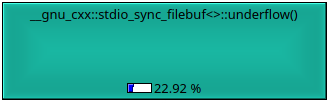
\includegraphics[scale=0.9]{underflow.png}
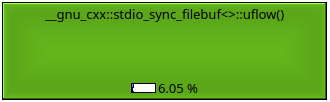
\includegraphics[scale=0.9]{Screenshot_20181117_002314.png}

\end{figure}


%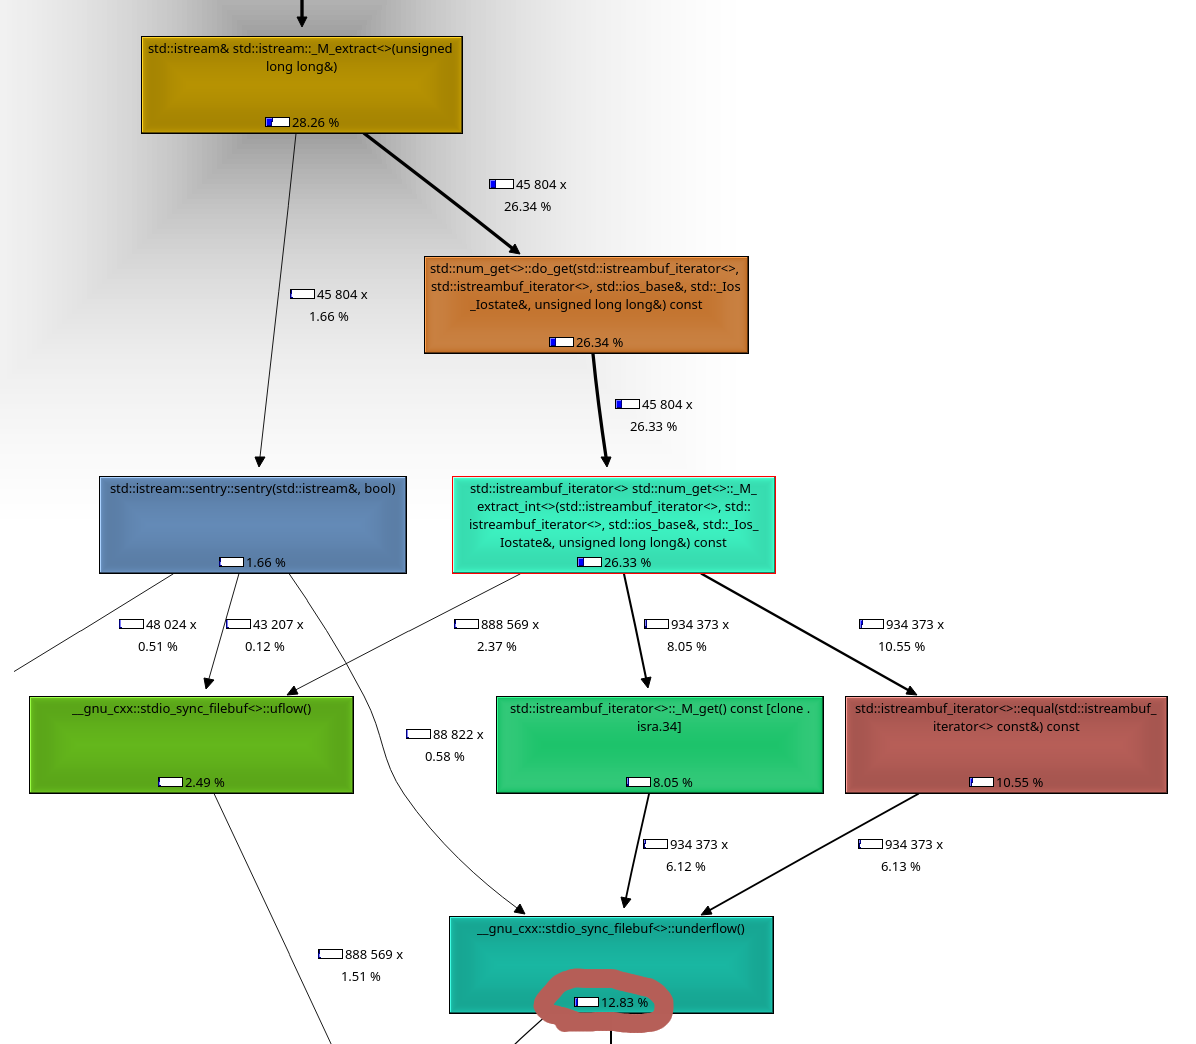
\includegraphics[scale=0.47]{sync.png}
\subsection*{Анализ потребления памяти}

Для анализа выделения памяти в программах используется модуль massif. Он собирает сведения не только о размерах блоков, выделяемых программой, но также и о том, сколько дополнительной памяти потребуется для хранения служебной информации.

После завершения программы под управлением massif, valgrind выдает краткую сводку использования памяти, а подробные данные выводятся в файл massif.out.<pid>. Для анализа этих данных может использоваться программа ms\_print. Эта программа может выдавать данные в виде псевдографических  графиков, демонстрирующих выделение памяти в программе в процессе работы, например вот так:
%\newpage
{\scriptsize
\begin{lstlisting}[label=massif,escapechar=!]
    MB
4.510^                                                                  #
|                                                                   @@@@#
|                                                               @@@@@@@@#
|                                                           @@@@@@@@@@@@#
|                                                       @@@@@@@@@@@@@@@@#
|                                                    @@@@@@@@@@@@@@@@@@@#
|                                                @@::@ @@@@@@@@@@@@@@@@@#
|                                             ::@@ ::@ @@@@@@@@@@@@@@@@@#
|                                        @@@@@: @@ ::@ @@@@@@@@@@@@@@@@@#
|                                     @@@@ @@@: @@ ::@ @@@@@@@@@@@@@@@@@#
|                                  @@@@@@@ @@@: @@ ::@ @@@@@@@@@@@@@@@@@#
|                              @:@@@@@@@@@ @@@: @@ ::@ @@@@@@@@@@@@@@@@@#
|                          @::@@:@ @@@@@@@ @@@: @@ ::@ @@@@@@@@@@@@@@@@@#
|                       @@@@: @@:@ @@@@@@@ @@@: @@ ::@ @@@@@@@@@@@@@@@@@#
|                   @@@@@@@@: @@:@ @@@@@@@ @@@: @@ ::@ @@@@@@@@@@@@@@@@@#
|               @:@@@ @@@@@@: @@:@ @@@@@@@ @@@: @@ ::@ @@@@@@@@@@@@@@@@@#
|           @:::@:@ @ @@@@@@: @@:@ @@@@@@@ @@@: @@ ::@ @@@@@@@@@@@@@@@@@#
|       @@@@@:::@:@ @ @@@@@@: @@:@ @@@@@@@ @@@: @@ ::@ @@@@@@@@@@@@@@@@@#
|    :::@@ @@:::@:@ @ @@@@@@: @@:@ @@@@@@@ @@@: @@ ::@ @@@@@@@@@@@@@@@@@#
|  :::::@@ @@:::@:@ @ @@@@@@: @@:@ @@@@@@@ @@@: @@ ::@ @@@@@@@@@@@@@@@@@#
0 +----------------------------------------------------------------------->Mi
0                                                                   433.6

Number of snapshots: 89
\end{lstlisting}
}

%Пользователь может использовать дополнительные опции massif для управления частотой снятия снапшотов, их количеством и списком функций, для которых будет производиться анализ.


\section*{perf}
Perf --- это незаменимый инструмент для анализа производительности отдельных программ и даже всей системы в целом. Начиная с версии ядра  Linux 2.6+ <<perf>> предоставляется как встроенный инструмент для статического профилирования. Работа утилиты основана на так называемых счётчиках производительности.

Счётчики производительности -- это регистры аппаратного обеспечения процессора, которые подсчитывают аппаратные события, такие как выполненные инструкции, ошибки кеша или неверные аргументы. Они составляют основу для профилирования приложений, отслеживания системных вызовов и определения узких мест. Perf обеспечивает богатую статистику выполнения программы. Среди прочего, для каждой задачи, для каждого процесса он описывает их счётчики рабочей нагрузки, выборку поверх них и аннотацию событий в дизассемблированном коде.

Контрольные точки -- это ключевые точки, размещенные в логически важных частях программы, например системные вызовы, события TCP / IP, операции файловой системы и т.д. 
Они практически не влияют на скорость исполнения кода, если не используются, и могут быть включены командой perf 
для сбора информации, включая временные метки и трассировки стека. perf также может динамически создавать точки трассировки, используя рамки kprobes и uprobes, для динамической трассировки ядра и пользовательского пространства.
\newline

Основные команды perf:
\begin{itemize}
\item perf stat: получить количество событий
\item perf record: запись событий для последующей отчетности
\item perf report: считывание отчёта, разбивка событий по процессам, функциям и т.д.
\item perf annotate: показ дизассемблированного кода с количеством событий
\item perf top: просмотр всех системных событий в реальном времени
\item perf bench: различные микробенчмарки ядра
\end{itemize}


Пример вывода \lstinline|perf stat| для тестируемой программы (1 000 000 команд вставки и удаления):
{ \footnotesize
\begin{lstlisting}
 Performance counter stats for './lab03':

3 763,48 msec task-clock:u                   #    0,990 CPUs utilized          
0      context-switches:u                    #    0,000 K/sec                  
0      cpu-migrations:u                      #    0,000 K/sec                  
8 671      page-faults:u                     # 2304,279 M/sec                  
6 953 488 887      cycles:u                  # 1847857,796 GHz                 
5 230 777 557      instructions:u            #    0,75  insn per cycle         
1 014 392 745      branches:u                # 269570221,897 M/sec             
32 393 045      branch-misses:u              # 3,19% of all branches        

3,803390643 seconds time elapsed

2,224674000 seconds user
1,533067000 seconds sys
\end{lstlisting}
}

Весь вывод \lstinline|perf record && perf report| приводить не вижу смысла, самое важное было получено при показе дизассемблированного кода и счётчиков для каждой функции. Как и ожидалось, функция Prefix(char const*, int, char const*, int) оказалось наиболее ``узким'' местом  в программе, \lstinline|perf| это услужливо показал:

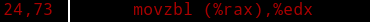
\includegraphics{mov.png} 

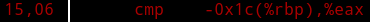
\includegraphics{cmp.png}

Путём 5-ти минутного поиска было выяснено, что инструкция mov обеспечивает разыменование объекта, расположенного по адесу, и записывает результат в указаный регистр. Инструкция movzbl работает точно так же, как mov, только расширяют один операнд до размера второго, знаково и беззнаково соответственно. Например, инструкция \lstinline|movzbl (%rdx, %rcx, 1),%esi| читайт байт (b) по адресу (\%rdx,\%rcx,1), расширяет его в длинное слово (l) путем добавления в начало нулей (z) и кладет результат в регистр \%esi.

Вторая инструкция осуществляет сравнение двух элементов (что нетрудно догадаться из названия)

Возможных путей усовершенствования данной функции я не вижу.

\section*{Gprof}

Gprof принадлежит к семейству гарантированных профилировщиков -- его работа обеспечивается компилятором (ключ --pg). При компиляции в начале и конце каждой функции расставляются контрольные точки. Разница между двумя этими точками и будет временем ее исполнения.

Стоит отметить, что <<gprof>> в данном случе точно <<знает>> и то, сколько раз была вызвана каждая функция. И хотя это может быть важным в некоторых ситуациях, это также имеет отрицательный эффект -- overhead от замеров может быть сравним или даже больше чем само тело функции.
\newline

Вот результат обработки с помощью <<gprof>> тестируемой программы:

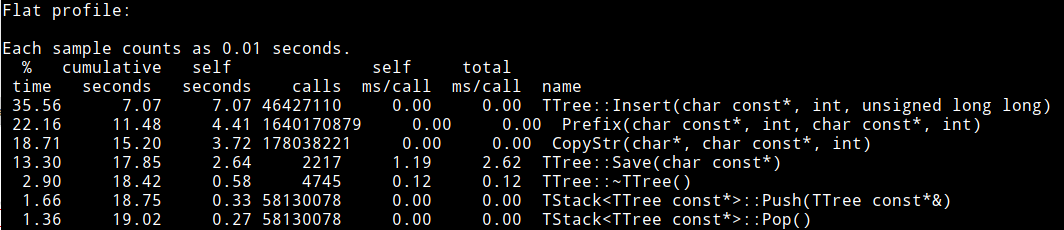
\includegraphics[scale=0.55]{gprof.png}

Это лишь часть вывода утилиты, на самом деле её вывод разделён на 2 большие части: данные профилирования и граф вызовов.


В части данных профилирования выводится информация о том, как много времени ваша программа затратила на выполнение каждой из функций, а также о том, как много раз эта функция была вызвана. Если вам нужно знать лишь о том, на какие функции была потрачена большая часть тактов центрального процессора, вы сможете найти в данной части всю необходимую информацию.

Граф вызовов описывает каждую из функций, выводя список вызывающих ее функций, список вызываемых из неё функций, а также информацию о количестве вызовов. Также в данной части присутствует оценочная информация, касающаяся времени, затрачиваемого в подфункциях каждой из функций. Данная информация позволяет обнаружить фрагменты кода, в которых можно попытаться сократить количество вызовов функций, использующих значительное количество процессорного времени.

По графу вызовов можно построить следующее изображение:

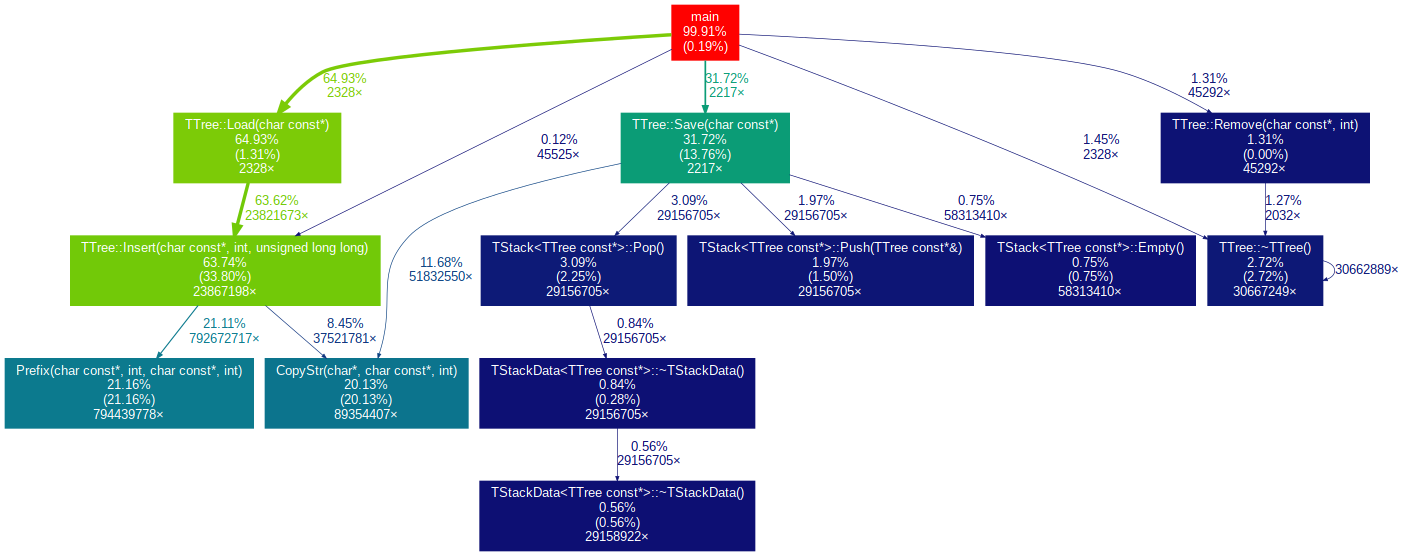
\includegraphics[scale=0.317]{outt.png}

\noindent Можно удостовериться, что количество вызовов функции совпадает с данными теста:

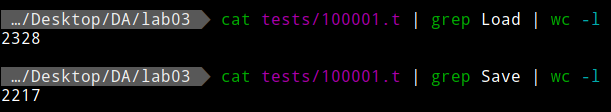
\includegraphics[scale=0.9]{tst.png}

\section*{Gcov}

Одним из популярных средств измерения покрытия кода тестами служит утилита gcov. Данная утилита используется совместно с gcc для анализа программ с целью достижения наибольшей производительности и эффективности кода, и выявления не покрываемых тестами участков кода. Предоставляемая статистика утилитой gcov, позволяет ответить на следующие вопросы:

\begin{itemize}
\item Как часто (количество прохождений) выполняется каждая строка кода.
\item Какие строки кода не выполняются.
\item Какой процент строк кода покрыт тестами для каждого файла.
\item Какой процент ветвлений (условий) покрыт тестами для каждого файла.
\end{itemize}

Для работы утилиты необходимо добавить следующие флаги компиляции:

\lstinline| -ftest-coverage -fprofile-arcs|

Далее необходимо обработать данные, появившиеся после исполнения в файлах: \lstinline|<filename>.gcno; <filename>.gcda| , где <filename> это имя файла с исходным кодом (без расширения cpp). И, собственно, сам запуск: \lstinline|gcov *.cpp|.
На выходе получаются файлы <filename>.cpp.gcov.

Их можно открыть как обычные текстовые файлы и оценить степень покрытия кода тестами. 

Проверка с помощью <<gcov>> тестируемой программы показала непокрытые тестами участки кода, в частности в функции удаления элемента из дерева:

{\scriptsize
\begin{lstlisting}
2354:   207:                delete node;
2354:   208:                break;
    -:  209:            } else {
#####:  210:                if (brother == nullptr) {
#####:  211:                    if (node->right == nullptr) {
#####:  212:                        delete[] node->key;
#####:  213:                        node->length = 0;
#####:  214:                        node->key = nullptr;
#####:  215:                        node->data = 0;
    -:  216:                    } else {
#####:  217:                        delete[] node->key; //! copy
#####:  218:                        brother = node->right;
#####:  219:                        node->key = new char[brother->length];
#####:  220:                        CopyStr(node->key, brother->key, brother->length);
#####:  221:                        node->length = brother->length;
#####:  222:                        node->data = brother->data;
#####:  223:                        node->right = brother->right;
#####:  224:                        node->left = brother->left;
#####:  225:                        brother->right = nullptr;
#####:  226:                        brother->left = nullptr;
#####:  227:                        delete brother;
    -:  228:                    }
    -:  229:                } else {
#####:  230:                    brother->right = temp;
#####:  231:                    node->right = nullptr;
#####:  232:                    node->left = nullptr;
#####:  233:                    delete node;
    -:  234:                }
    -:  235:            }
#####:  236:            break;
1810240:  237:        } else if (prefix == 0) {
1693584:  238:            brother = node;
\end{lstlisting}}

Этот кусок кода обрабатывает удаление из корня, и был проверен на специальных тестах, написанных вручную.

\section*{Выводы}

Профилирование и тестирование заняло примерно столько же времени, чем написание самой программы. Но хочу сказать, что профилирование мне понравилось намного больше. Я получил много информации о том, как и почему может тормозить программа и как точно найти место, где она течёт по памяти или долго выполняется. Огромное удовольствие доставила утилита <<gcov>>, так как она позволяет увидеть слабые места в сгенерированных тестах и гарантированно проверить весь код. Были получены навыки работы с различными профилировщиками, они сильно различались по способу реализации и предложенному функционалу, но все они оказались необычайно полезными при проверке качества кода. Ведь не всегда просто найти в коде ``узкие'' места или утечку памяти. Я был невероятно впечатлён работой утилиты valgrind, её создатели провели очень сложную работу и результат их трудов я всегда использую при проверке кода на ошибки и для создания статистики её работы. Также очень понравилось визуализировать вывод callgrind и gprof при помощи kcachegrind и gprof2dot, но для себя я выяснил, что в принципе никому такие красивые графики/диаграммы/графы не нужны, разве что для презентации или огромного проекта с миллионами функций. Но никак не для лабораторных работ размером меньше двух тысяч строк кода.
\pagebreak


\end{document}
